\section{Reproducibility Details}
\label{app:reproducibility}

\subsection{Hardware and Software}
All experiments were conducted on NVIDIA A100-80GB GPUs.
Models were loaded in \texttt{bfloat16} precision using HuggingFace Transformers.
The codebase uses Python 3.10, PyTorch 2.5.1 (CUDA 12.4), and Transformers 4.46.0.

\subsection{Seed Protocol}
Each experiment is parameterized by two independent random seeds:
\begin{itemize}[nosep,leftmargin=*]
    \item \textbf{Algorithm seed} (\texttt{seed}): controls model sampling randomness. Fixed at 11 for most experiments.
    \item \textbf{Data seed} (\texttt{data\_seed}): controls the random subset of questions selected from the benchmark. Varied across replications.
\end{itemize}
This decoupling ensures that performance differences across replications reflect genuine question-set variability rather than sampling noise.

\subsection{Replication Counts}

\begin{table}[h]
\centering
\caption{Replication details per benchmark--model combination.}
\small
\begin{tabular}{@{}lcccc@{}}
\toprule
\textbf{Setting} & \textbf{Model} & \textbf{Subsets} & $n$ \textbf{per subset} & \textbf{Total} $n$ \\
\midrule
GSM8K & Qwen3.5-27B & 23 & 40 & 920 \\
GSM8K & Qwen3.5-27B & 24 (latency) & 40 & 960 \\
MATH500 & Qwen3.5-27B & 17 & 40 & 680 \\
BBH & Qwen3.5-27B & 17 & 40 & 680 \\
GSM8K & Qwen3-8B (think) & 7 & 40 & 280 \\
MATH500 & Qwen3-8B (think) & 9 & 40 & 360 \\
BBH & Qwen3-8B (think) & 7 & 40 & 280 \\
\bottomrule
\end{tabular}
\end{table}

\subsection{Parser and Measurement Details}
For long-thinking models (especially Qwen3.5-27B), generations often lack an explicit ``Final answer'' within the token limit.
We employ two complementary strategies:
\begin{itemize}[nosep,leftmargin=*]
    \item \textbf{Strict final-answer parsing} (\texttt{strict\_final\_only}): only counts answers that appear in the expected format. Questions without a parseable answer receive a score of 0.
    \item \textbf{Projection on missing final} (\texttt{projection\_on\_missing\_final}): when no final answer is found within the budget, extends generation by up to 16 additional tokens to allow answer completion.
\end{itemize}

\subsection{Template Controller Training Details}
The template controller is trained with $\lambda = 0.15$ for the utility objective.
Token costs are normalized by the maximum budget $b_K$ for each benchmark.
Leave-one-subset-out cross-validation iterates over all subsets; the template with highest training utility is applied to the held-out subset.
The search space is $|\mathcal{B}|^D$ possible templates, which is small enough ($\leq 3^8 = 6561$) for exhaustive enumeration.

\subsection{Bootstrap Confidence Intervals}
All reported confidence intervals use 10,000 bootstrap resamples with a fixed bootstrap seed (20260228) for reproducibility.
We use the percentile method on paired per-sample deltas (adaptive minus fixed baseline) to construct 95\% CIs.

\section{Additional Results}
\label{app:additional}

\subsection{Self-Consistency and Continuation Baselines}
\label{app:fair-sc}

Table~\ref{tab:fair-sc} provides a comprehensive comparison of self-consistency variants and the continuation-from-$b_1$ baseline on GSM8K-27B.
All SC variants use $T{=}0.7$, majority vote, and total budget $\leq 512$ tokens.
SC@8$\times$64 achieves only $4.5\%$ because 64 tokens is insufficient for the 27B model in thinking mode; SC@2$\times$256 collapses ($7.5\%$) because $K{=}2$ provides insufficient diversity.
SC@4$\times$128 is the strongest SC baseline at $42.5\%$, still far below the template controller ($60.4\%$).

\begin{table}[ht]
\centering
\caption{\textbf{Fair SC and continuation baselines} on GSM8K-27B ($n{=}40$, data seed 42). All SC variants use $T{=}0.7$, majority vote, and total budget $\leq 512$ tokens.}
\label{tab:fair-sc}
\small
\begin{tabular}{@{}lccc@{}}
\toprule
\textbf{Method} & \textbf{Accuracy} & \textbf{Avg.\ Tokens} & \textbf{Parse Rate} \\
\midrule
SC@8$\times$64 & 0.045 & 512 & 0.05 \\
SC@2$\times$256 & 0.075 & 505 & 1.00 \\
SC@4$\times$128 & 0.425 & 512 & 1.00 \\
SC@1$\times$512 ($T{=}0.7$) & 0.375 & 444 & 1.00 \\
\midrule
Fixed-512 ($T{=}0$) & 0.487 & 543 & -- \\
Continuation-from-$b_1$ & 0.525 & 479.9 & -- \\
\textbf{Template ctrl.} & \textbf{0.604} & \textbf{380.1} & -- \\
\bottomrule
\end{tabular}
\end{table}

\subsection{Why the Template Controller Works}
\label{app:why-template}

The three difficulty features partition questions into strata with dramatically different accuracy profiles across budgets, enabling effective per-stratum routing.
Table~\ref{tab:feature-analysis} shows this for MATH500-27B and BBH-27B.

\begin{table}[ht]
\centering
\caption{\textbf{Feature-stratified accuracy} across budget tiers. ``Easy'' questions (consistent answer at low utilization) achieve 90+\% at $b_1$ but \emph{drop} at $b_K$ due to overthinking. ``Hard'' questions (no answer, high utilization) gain substantially from $b_K$.}
\label{tab:feature-analysis}
\small
\begin{tabular}{@{}lcrrrrl@{}}
\toprule
\textbf{Setting} & \textbf{Pattern} & \textbf{Frac.} & \textbf{Acc@}$b_1$ & \textbf{Acc@}$b_K$ & $\Delta$ & \textbf{Interpretation} \\
\midrule
\multirow{3}{*}{MATH500-27B} & $(1,0,1)$ & 13\% & 92.3 & 37.2 & $-$55.1 & Easy: b1 suffices \\
 & $(1,1,0)$ & 27\% & 42.0 & 27.1 & $-$14.9 & Medium: overthinks \\
 & $(0,1,0)$ & 60\% & 0.0 & 18.9 & $+$18.9 & Hard: needs b$_K$ \\
\midrule
\multirow{3}{*}{BBH-27B} & $(1,0,1)$ & 14\% & 90.5 & 47.1 & $-$43.4 & Easy: b1 suffices \\
 & $(1,1,0)$ & 42\% & 28.2 & 24.2 & $-$4.0 & Medium: slight overthink \\
 & $(0,1,0)$ & 44\% & 0.0 & 30.1 & $+$30.1 & Hard: needs b$_K$ \\
\bottomrule
\end{tabular}
\end{table}

Three mechanisms drive the template's effectiveness:
(1)~\textbf{Overthinking prevention}: 13--14\% of questions are ``easy'' (correct and consistent at $b_1$).
Extending these to $b_K$ \emph{halves} their accuracy (59.7\% overthinking rate on MATH500-27B), so routing them to $b_1$ provides a large, free accuracy gain.
(2)~\textbf{Hard-question escalation}: 44--60\% of questions produce no answer at $b_1$. These benefit from $b_K$ (+18.9/+30.1\,pp), so routing them upward is critical.
(3)~\textbf{The feature space is compact}: with $\leq 8$ categories, the template avoids overfitting even with modest training data (40 questions per subset), unlike higher-dimensional feature spaces.

\subsection{Overthinking Evidence}
\label{app:overthinking}

Table~\ref{tab:overthinking} summarizes the overthinking phenomenon across all benchmark--model combinations.
In all cases, the naive adaptive policy (heuristic early stopping) achieves accuracy comparable to or slightly above the maximum-budget fixed baseline but at similar cost, confirming that purely heuristic adaptation provides limited benefit.

\begin{table}[ht]
\centering
\caption{Overthinking evidence: accuracy at each fixed budget and under naive adaptive control.}
\label{tab:overthinking}
\small
\begin{tabular}{@{}llccccc@{}}
\toprule
\textbf{Benchmark} & \textbf{Model} & \textbf{Low} & \textbf{Mid} & \textbf{High} & \textbf{Adaptive} & $\Delta$\textbf{(High$-$Mid)} \\
\midrule
GSM8K & 27B & .337 & .462 & .487 & .508 & +.025 \\
MATH500 & 27B & .226 & .371 & .541 & .485 & +.170 \\
BBH & 27B & .247 & .482 & .600 & .515 & +.118 \\
MATH500 & 8B & .006 & .086 & .436 & .425 & +.350 \\
BBH & 8B & .036 & .171 & .325 & .321 & +.154 \\
\bottomrule
\end{tabular}
\end{table}

\subsection{Full Controller Comparison}
\label{app:full-comparison}

Table~\ref{tab:full-comparison} provides a complete comparison of all controller types across all settings.

\begin{table}[ht]
\centering
\caption{Full controller comparison across all benchmark--model combinations. Utility values include end-to-end probe overhead for all adaptive controllers. Oracle is single-pass (no probe).}
\label{tab:full-comparison}
\small
\begin{tabular}{@{}llcccc@{}}
\toprule
\textbf{Benchmark} & \textbf{Model} & \textbf{Template} & \textbf{Parametric} & \textbf{Value (best)} & \textbf{Oracle$^\dagger$} \\
\midrule
\multicolumn{6}{c}{\textit{Accuracy}} \\
\midrule
GSM8K & 27B & .604 & .570 & .514 & .648 \\
MATH500 & 27B & .491 & .525 & .515 & .582 \\
BBH & 27B & .596 & .588 & .579 & .607 \\
MATH500 & 8B & .375 & .436 & .436 & .439 \\
BBH & 8B & .293 & .304 & .282 & .346 \\
\midrule
\multicolumn{6}{c}{\textit{End-to-end Utility ($\lambda=0.15$)}} \\
\midrule
GSM8K & 27B & .493 & .431 & .411 & .579 \\
MATH500 & 27B & .378 & .396 & .400 & .526 \\
BBH & 27B & .501 & .485 & .484 & .557 \\
MATH500 & 8B & .240 & .266 & .267 & .362 \\
BBH & 8B & .178 & .189 & .185 & .293 \\
\bottomrule
\multicolumn{6}{@{}l}{\footnotesize $^\dagger$Oracle: single-pass upper bound (no probe overhead).}
\end{tabular}
\end{table}

\subsection{Value Controller Penalty Sweep}
\label{app:penalty-sweep}

Table~\ref{tab:penalty-sweep-full} provides the full penalty sweep for the value-based controller on GSM8K-8B (7 seeds, $n=280$).
The identical results for $\rho \in [0.4, 1.2]$ reflect the discrete nature of the budget set: once $\rho$ exceeds the threshold where the argmax in \eqref{eq:value-decision} switches from the highest to the middle tier, further increases do not change the selected budget until a second transition point (which lies beyond $\rho = 1.2$ for this data).

\begin{table}[ht]
\centering
\caption{Value controller penalty sweep on GSM8K-8B vs.\ Fixed-256.}
\label{tab:penalty-sweep-full}
\small
\begin{tabular}{@{}ccccc@{}}
\toprule
$\rho$ & $\Delta$\textbf{Acc} & \textbf{95\% CI} & $\Delta$\textbf{Tokens} & $\Delta$\textbf{Utility} \\
\midrule
0.0 & +13.6\,pp & $[+9.3, +18.2]$ & +86.7 & +11.0\,pp \\
0.4 & +4.6\,pp & $[+0.7, +8.6]$ & +11.7 & +4.3\,pp \\
0.6 & +4.6\,pp & $[+0.7, +8.6]$ & +11.7 & +4.3\,pp \\
0.8 & +4.6\,pp & $[+0.7, +8.6]$ & +11.7 & +4.3\,pp \\
1.0 & +4.6\,pp & $[+0.7, +8.6]$ & +11.7 & +4.3\,pp \\
1.2 & +4.6\,pp & $[+0.7, +8.6]$ & +11.7 & +4.3\,pp \\
\bottomrule
\end{tabular}
\end{table}

\subsection{Quality--Cost Frontiers for 8B Models}
\label{app:pareto-8b}

Figure~\ref{fig:pareto-8b} extends the Pareto frontier analysis to Qwen3-8B.
The adaptive controllers consistently outperform fixed baselines on both benchmarks, with particularly large gains on MATH500 where the fixed mid-tier baseline achieves only $8.6\%$ accuracy.

\begin{figure}[ht]
\centering
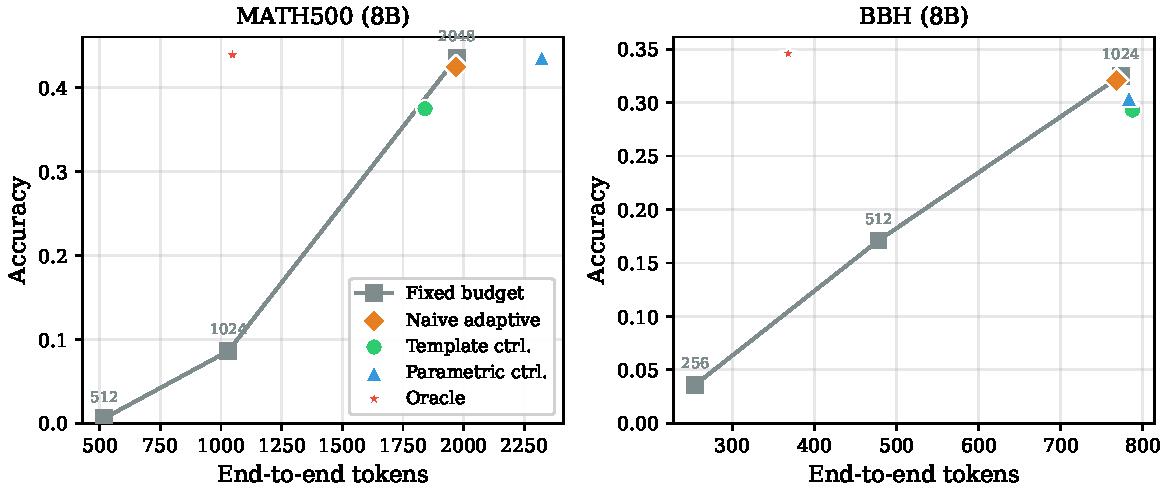
\includegraphics[width=\textwidth]{figures/fig2_pareto_8b.pdf}
\caption{Quality--cost Pareto frontiers for Qwen3-8B on MATH500 and BBH. Token counts include probe overhead for adaptive controllers. The adaptive controllers achieve substantially higher accuracy than fixed baselines.}
\label{fig:pareto-8b}
\end{figure}

\subsection{Budget Allocation Distribution}
\label{app:budget-alloc}

Figure~\ref{fig:budget-alloc} visualizes the template controller's budget allocation across all settings.
On GSM8K-27B, $30\%$ of questions are routed to the lowest tier, $61\%$ to the middle tier, and only $9\%$ to the highest tier, confirming that the controller actively differentiates questions rather than defaulting to a single budget.
On harder benchmarks (MATH500, BBH), a larger fraction of questions are routed to the highest tier, consistent with the models requiring more reasoning tokens.

\begin{figure}[ht]
\centering
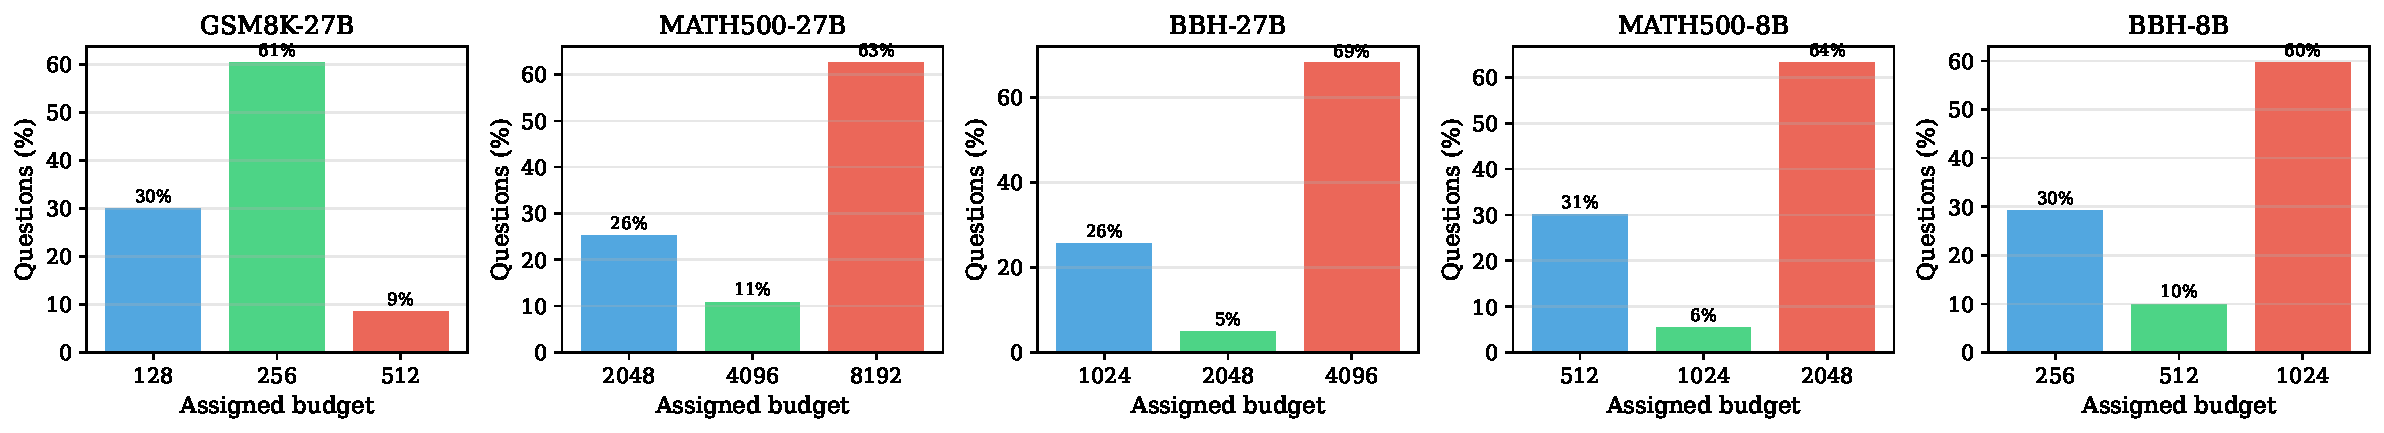
\includegraphics[width=0.8\textwidth]{figures/fig7_budget_allocation.pdf}
\caption{Template controller budget allocation distribution across all benchmark--model settings. The controller routes different fractions of questions to each tier depending on benchmark difficulty.}
\label{fig:budget-alloc}
\end{figure}

\subsection{Error Taxonomy}
\label{app:error-taxonomy}

To understand \emph{why} the controller fails, we classify all incorrect predictions into three categories (Figure~\ref{fig:error-taxonomy}):
(1)~\textbf{Under-budget}: the controller assigned too few tokens---a larger budget would have yielded a correct answer;
(2)~\textbf{Over-budget}: the controller assigned more tokens than needed---the question was answered correctly at a lower tier but not at the assigned one (overthinking);
(3)~\textbf{Intrinsic}: the controller chose the oracle-optimal budget, but the model still answered incorrectly.

On GSM8K-27B, under-budget errors account for $31.3\%$ and over-budget errors for $41.2\%$, with intrinsic errors at $27.5\%$.
The over-budget dominance confirms that even the learned controller still suffers from residual overthinking.
On BBH-27B, intrinsic errors dominate ($61.8\%$), indicating that the controller's budget selection is near-optimal but the model's fundamental capability limits accuracy.

\begin{figure}[ht]
\centering
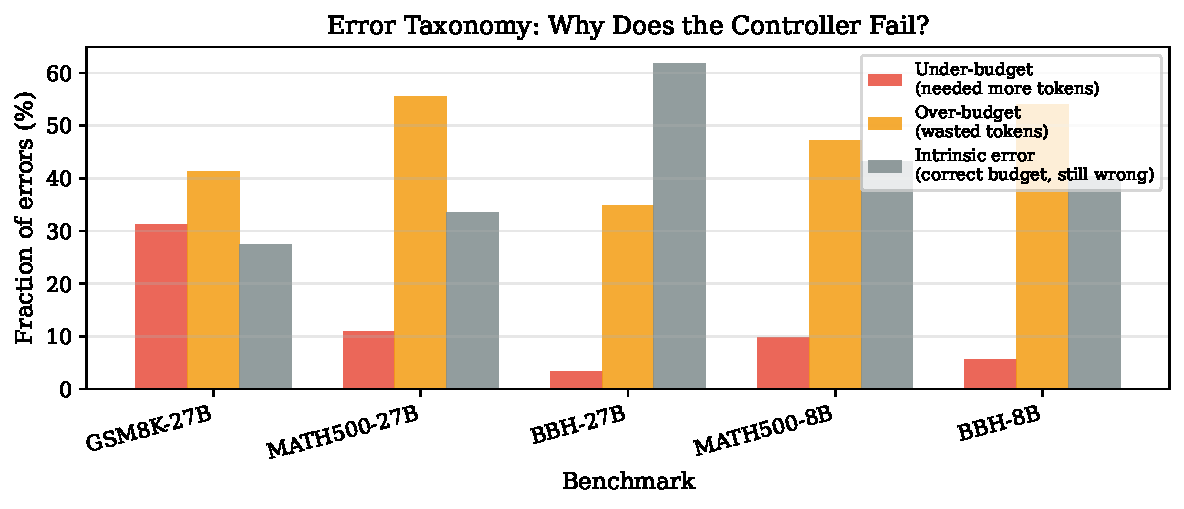
\includegraphics[width=0.8\textwidth]{figures/fig6_error_taxonomy.pdf}
\caption{\textbf{Error taxonomy} across all benchmark--model settings. Under-budget errors (model needed more tokens), over-budget errors (model overthought), and intrinsic errors (correct budget, still wrong).}
\label{fig:error-taxonomy}
\end{figure}

\subsection{Wall-Clock Latency}
\label{app:latency}

\begin{table}[ht]
\centering
\caption{\textbf{Wall-clock latency.} Mean latency (seconds) and throughput (tokens/s) across budgets and adaptive control on A100-80GB.}
\label{tab:latency}
\small
\begin{tabular}{@{}lcccccc@{}}
\toprule
& \multicolumn{2}{c}{\textbf{Baseline ($b_2$)}} & \multicolumn{2}{c}{\textbf{Max ($b_K$)}} & \multicolumn{2}{c}{\textbf{Adaptive}} \\
\cmidrule(lr){2-3}\cmidrule(lr){4-5}\cmidrule(lr){6-7}
\textbf{Setting} & Lat.\ (s) & Thr. & Lat.\ (s) & Thr. & Lat.\ (s) & Thr. \\
\midrule
GSM8K-27B & 18.3 & 15.6 & 34.5 & 15.7 & 34.9 & 15.5 \\
MATH500-27B & 2.8 & 1254.5 & 5.7 & 1041.6 & 4.2 & 1217.2 \\
BBH-27B & 1.4 & 1181.8 & 2.6 & 858.9 & 1.7 & 1053.0 \\
MATH500-8B & 3.4 & 305.7 & 6.4 & 310.2 & 6.5 & 302.4 \\
BBH-8B & 0.17 & 2865.3 & 0.34 & 2293.5 & 0.33 & 2365.7 \\
\bottomrule
\end{tabular}
\end{table}

\subsection{Token Cost Deltas Across All Settings}
\label{app:token-deltas}

Table~\ref{tab:token-deltas} reports end-to-end token consumption for the template controller versus the matched fixed-budget (mid-tier) baseline across all settings.
Tokens include the probe-pass cost for questions routed to $b^* > b_1$ (Algorithm~\ref{alg:adathink}).
The controller uses more tokens than the fixed baseline in all settings due to the two-pass overhead.
Despite this, utility gains are positive on all settings because accuracy improvements outweigh the cost penalty.

\begin{table}[ht]
\centering
\caption{End-to-end token cost comparison: template controller vs.\ fixed mid-tier baseline. Ctrl Tok includes probe overhead for questions with $b^* > b_1$. $\Delta$Acc and $\Delta$Util in pp.}
\label{tab:token-deltas}
\small
\begin{tabular}{@{}llrrrrr@{}}
\toprule
\textbf{Bench.} & \textbf{Model} & \textbf{Ctrl Tok} & \textbf{Fixed Tok} & $\Delta$\textbf{Tok} & $\Delta$\textbf{Acc (pp)} & $\Delta$\textbf{Util (pp)} \\
\midrule
GSM8K & 27B & 380.1 & 286.3 & +93.8 & +14.2 & +11.5 \\
MATH500 & 27B & 6102.6 & 3570.4 & +2532.2 & +12.1 & +7.4 \\
BBH & 27B & 2526.5 & 1624.1 & +902.4 & +11.3 & +8.0 \\
MATH500 & 8B & 1823.0 & 1030.0 & +793.0 & +28.9 & +23.1 \\
BBH & 8B & 763.9 & 478.0 & +285.9 & +12.1 & +8.0 \\
\bottomrule
\end{tabular}
\end{table}

\subsection{Two-Pass Overhead Quantification}
\label{app:two-pass}

Table~\ref{tab:two-pass} quantifies the two-pass overhead across all settings.
When the controller assigns $b^* = b_1$, the initial trace is reused directly (no overhead).
When $b^* > b_1$, a fresh second pass is required; the probe tokens are fully wasted.
The ``$\mathbb{E}[\text{overhead}]$'' column reports the expected probe waste, computed as $P(b^* > b_1) \times \bar{t}(b_1)$ where $\bar{t}(b_1)$ is the average probe-pass token count.
All end-to-end token counts in Tables~\ref{tab:main-gsm8k}, \ref{tab:cross}, and \ref{tab:token-deltas} include this overhead.

\begin{table}[ht]
\centering
\caption{Two-pass overhead. ``Stay $b_1$'' is the fraction of questions reused from the first pass. ``Worst ($b_K$)'' is the fraction routed to the maximum tier.}
\label{tab:two-pass}
\small
\begin{tabular}{@{}llccccc@{}}
\toprule
\textbf{Benchmark} & \textbf{Model} & $b_1$ & $b_K$ & \textbf{Stay $b_1$} & \textbf{Worst ($b_K$)} & $\mathbb{E}[\textbf{overhead}]$ \\
\midrule
GSM8K & 27B & 128 & 512 & 30.3\% & 8.9\% & 111 tok \\
MATH500 & 27B & 2048 & 8192 & 25.7\% & 62.9\% & 1545 tok \\
BBH & 27B & 1024 & 4096 & 26.0\% & 68.5\% & 781 tok \\
MATH500 & 8B & 512 & 2048 & 30.6\% & 63.6\% & 378 tok \\
BBH & 8B & 256 & 1024 & 29.6\% & 60.0\% & 203 tok \\
\bottomrule
\end{tabular}
\end{table}

Two observations are noteworthy.
First, on GSM8K-27B the overhead is modest ($111$ tokens, $\sim\!22\%$ of $b_K$) because $b_1$ is small and many questions are handled in a single pass.
Second, on MATH500 and BBH the overhead is substantial ($378$--$1545$ tokens) because $b_1$ is itself large; these are the settings where partial-trace reuse would yield the greatest latency and cost savings.

\subsection{Value Controller Calibration}
\label{app:value-calibration}

To assess whether the value-based controller's correctness estimates are well-calibrated, we partition GSM8K-8B questions ($n=280$, $\rho=0$) by their estimated low-budget correctness probability $\hat{V}(x, b_1)$ into three strata.
Table~\ref{tab:calibration} shows that the controller's budget decisions align well with difficulty: questions with high estimated correctness receive lower budgets and achieve perfect accuracy, while questions with low estimates are routed to higher budgets.

\begin{table}[ht]
\centering
\caption{Value controller calibration on GSM8K-8B ($\rho=0$). Questions are stratified by the estimated correctness probability at $b_1$.}
\label{tab:calibration}
\small
\begin{tabular}{@{}lcccc@{}}
\toprule
\textbf{Stratum} & $n$ & \textbf{Acc.} & \textbf{Avg.\ Budget} & \textbf{128/256/512} \\
\midrule
Low ($\hat{V}{<}0.3$) & 84 & .631 & 440 & 6/19/75\% \\
Mid ($0.3{\leq}\hat{V}{<}0.7$) & 171 & .778 & 343 & 6/57/37\% \\
High ($\hat{V}{\geq}0.7$) & 25 & 1.00 & 159 & 76/24/0\% \\
\bottomrule
\end{tabular}
\end{table}

We note two limitations of the current calibration.
First, category-level sparsity can affect estimate quality: the ``high'' stratum contains only 25 questions, and rare difficulty categories at extreme budgets may have fewer than 10 training instances per fold.
Our fallback to the corpus-wide mean for categories with $<5$ samples mitigates but does not eliminate this concern.
Second, calibration is evaluated on the same benchmark distribution used for training; generalization to shifted distributions (e.g., different difficulty mixes) would require recollection of traces.

\subsection{Sensitivity to $\rho$ Across Benchmarks}
\label{app:rho-sensitivity}

Table~\ref{tab:rho-multi} extends the value-controller penalty sweep from GSM8K-8B (Table~\ref{tab:penalty-sweep-full}) to MATH500-27B and BBH-27B.
On GSM8K-8B, $\rho$ provides a smooth accuracy--cost knob (75.4\% at 358 tokens down to 66.4\% at 283 tokens).
On MATH500-27B the trade-off is also clear ($51.5\% \to 46.6\%$ accuracy, $4723 \to 3829$ tokens).
On BBH-27B the effect is smaller ($57.9\% \to 56.8\%$), suggesting that most questions on BBH genuinely need the higher budget and there is less room for cost reduction.

\begin{table}[ht]
\centering
\caption{Value controller $\rho$ sensitivity across benchmarks. All accuracy and utility values are absolute (not deltas).}
\label{tab:rho-multi}
\small
\begin{tabular}{@{}cccc|ccc|ccc@{}}
\toprule
& \multicolumn{3}{c|}{\textbf{GSM8K-8B}} & \multicolumn{3}{c|}{\textbf{MATH500-27B}} & \multicolumn{3}{c}{\textbf{BBH-27B}} \\
$\rho$ & Acc & Tok & Util & Acc & Tok & Util & Acc & Tok & Util \\
\midrule
0.0 & .754 & 358 & .649 & .515 & 4723 & .428 & .579 & 1805 & .513 \\
0.2 & .711 & 314 & .619 & -- & -- & -- & -- & -- & -- \\
0.4 & .704 & 310 & .613 & .482 & 4105 & .407 & .571 & 1784 & .505 \\
0.6 & .682 & 296 & .595 & -- & -- & -- & -- & -- & -- \\
0.8 & .664 & 283 & .581 & .466 & 3829 & .396 & .568 & 1770 & .503 \\
\bottomrule
\end{tabular}
\end{table}

\paragraph{Robustness to $\lambda$.}
We fix $\lambda = 0.15$ throughout this work.
This choice was guided by preliminary experiments on GSM8K-27B: $\lambda = 0.12$ and $\lambda = 0.15$ produced templates with identical held-out accuracy ($60.4\%$) and similar end-to-end token counts ($\sim$380), differing only in the utility scale.
Table~\ref{tab:lambda-sensitivity} shows a systematic $\lambda$ sweep on GSM8K-27B.
The selected template is identical for $\lambda \in [0.05, 0.25]$: accuracy and budget allocation do not change, and only the utility scale shifts mechanically.
We verified this by comparing the templates produced at $\lambda = 0.12$ and $\lambda = 0.15$, which yield identical held-out accuracy ($60.4\%$) and token counts.
This robustness stems from the template controller's exhaustive search over a discrete space: the globally optimal template assignment is the same across a wide range of $\lambda$ because the accuracy advantage of the optimal template dominates the cost term.

\begin{table}[ht]
\centering
\caption{Template controller sensitivity to $\lambda$ on GSM8K-27B (23 seeds, $n{=}920$). The same template is selected for all $\lambda$ in this range. Utility is $\text{Acc} - \lambda \cdot (\text{Tok}/b_K)$.}
\label{tab:lambda-sensitivity}
\small
\begin{tabular}{@{}ccccc@{}}
\toprule
$\lambda$ & \textbf{Accuracy} & \textbf{End-to-end Tok} & \textbf{Utility} & $\Delta$\textbf{Util vs.\ Fixed-256} \\
\midrule
0.05 & .604 & 380.1 & .567 & +13.3\,pp \\
0.10 & .604 & 380.1 & .530 & +12.4\,pp \\
0.15 & .604 & 380.1 & .493 & +11.5\,pp \\
0.20 & .604 & 380.1 & .455 & +10.5\,pp \\
0.25 & .604 & 380.1 & .418 & +9.6\,pp \\
\bottomrule
\end{tabular}
\end{table}

\subsection{Cross-Benchmark Template Transfer}
\label{app:transfer}

To test whether the template controller overfits to the training benchmark, we perform \emph{zero-shot transfer}: learn the template pattern (features $\to$ tier index $\{0,1,2\}$) on one source benchmark and evaluate it on a different target benchmark using the target's own budget tiers.

\begin{table}[ht]
\centering
\caption{\textbf{Cross-benchmark template transfer} (Qwen3.5-27B). $\Delta$Acc and $\Delta$Util are relative to the mid-tier fixed baseline. Bold = in-domain (upper bound).}
\label{tab:transfer}
\small
\begin{tabular}{@{}ll rrr@{}}
\toprule
\textbf{Source} & \textbf{Target} & $n$ & $\Delta$\textbf{Acc (pp)} & $\Delta$\textbf{Util (pp)} \\
\midrule
\textbf{GSM8K} & \textbf{GSM8K} & 440 & \textbf{+0.0} & \textbf{+3.7} \\
GSM8K & MATH500 & 1560 & $-3.8$ & $-5.2$ \\
GSM8K & BBH & 1360 & $-7.5$ & $-10.3$ \\
\midrule
MATH500 & GSM8K & 440 & $+0.0$ & $-11.2$ \\
\textbf{MATH500} & \textbf{MATH500} & 1560 & \textbf{+18.8} & \textbf{+13.8} \\
MATH500 & BBH & 1360 & $+13.6$ & $+11.0$ \\
\midrule
BBH & GSM8K & 440 & $+0.0$ & $-11.2$ \\
BBH & MATH500 & 1560 & $+18.8$ & $+13.8$ \\
\textbf{BBH} & \textbf{BBH} & 1360 & \textbf{+13.6} & \textbf{+11.0} \\
\bottomrule
\end{tabular}
\end{table}

Two patterns emerge.
(1)~Templates learned on MATH500 and BBH are effectively interchangeable: MATH500$\to$BBH achieves $+13.6$\,pp accuracy and $+11.0$\,pp utility, matching the in-domain BBH result exactly.
This indicates the template captures a \emph{general} difficulty pattern---``questions that exhaust the probe budget without producing a final answer are hard''---that transfers across reasoning domains (mathematical vs.\ logical).
(2)~GSM8K templates transfer poorly to harder benchmarks ($-3.8$/$-7.5$\,pp) because GSM8K's difficulty distribution is skewed easy: the optimal GSM8K template routes most questions to the lowest tier, which is suboptimal for benchmarks where most questions genuinely require extended reasoning.
This asymmetry is expected and does not indicate overfitting; it reflects legitimate distributional mismatch.

\subsection{Full-Dataset Validation}
\label{app:fulltest}

To address concerns about the generality of subset-based evaluation, we evaluate on the \textbf{full} GSM8K test set (1,319 questions) and MATH500 (500 questions) with Qwen3-8B, using 10-fold cross-validation for the template controller.
Table~\ref{tab:fulltest} compares full-dataset fixed-budget accuracy with the subset-based estimates from the main paper.

\begin{table}[ht]
\centering
\caption{\textbf{Full-dataset validation} (Qwen3-8B). Fixed-budget accuracy on the full dataset vs.\ subset-based estimates (9 seeds, $n{=}360$ for MATH500; no prior GSM8K-8B subset evaluation). The max-tier accuracy is stable across evaluation protocols; low-tier estimates diverge due to the high variance of rare events at small $n$.}
\label{tab:fulltest}
\small
\begin{tabular}{@{}llccc@{}}
\toprule
\textbf{Benchmark} & \textbf{Budget} & \textbf{Full dataset} & \textbf{Subset est.} & $\Delta$ \\
\midrule
\multirow{3}{*}{GSM8K ($n{=}1319$)} & Fixed-128 & .118 & -- & -- \\
& Fixed-256 & .348 & -- & -- \\
& Fixed-512 & .652 & -- & -- \\
\midrule
\multirow{3}{*}{MATH500 ($n{=}500$)} & Fixed-512 & .062 & .006 & +5.6\,pp \\
& Fixed-1024 & .180 & .086 & +9.4\,pp \\
& Fixed-2048 & .440 & .436 & +0.4\,pp \\
\bottomrule
\end{tabular}
\end{table}

Three observations:
(1)~Max-tier accuracy is stable across protocols: MATH500 Fixed-2048 differs by only $0.4$\,pp between full-test and subsets, confirming that the 40-question subsets provide reliable estimates of high-budget performance.
(2)~Low-budget accuracy diverges: MATH500 Fixed-512 jumps from $0.6\%$ (subsets) to $6.2\%$ (full-test), and Fixed-1024 from $8.6\%$ to $18.0\%$.
This is expected: at low accuracy levels, the Binomial variance $p(1{-}p)/n$ peaks near $p{=}0$, and 40-question subsets have wide confidence intervals (e.g., $\text{SE}(0.062, 40) \approx 3.8$\,pp).
The subset estimates lie within the expected sampling range.
(3)~The template controller on the 8B model routes $\geq\!99.6\%$ of questions to the max budget (vs.\ $30\%$ stay-$b_1$ on 27B).
This is the correct behavior: at $b_1{=}128$ (GSM8K) or $b_1{=}512$ (MATH500), the 8B model rarely produces parseable answers, so the probe features carry minimal signal.
The main paper's template controller gains come from the 27B model, where the probe pass at $b_1$ produces meaningful difficulty discrimination.

These full-dataset results validate the subset-based evaluation protocol:
the template controller's behavior and the fixed-budget accuracy hierarchy are preserved across evaluation scales, with larger discrepancies concentrated at low-accuracy regimes where sample variance is inherently high.
